
% pnu_sampleKor.tex v1.0
% 본 양식은 서울대학교 전기컴퓨터공학부 학위논문 양식을 활용하여, 부산대학교의 양식에 맞춘 것입니다.
% https://ee.snu.ac.kr/community/notice/academic?bm=v&bbsidx=48811

% 논문작성을 위해서 한글패키지가 설치되어 있어야 합니다.
% MikTeX 을 사용할 것을 권장하며, MikTeX의 설치 및 한글 패키지와 관련된 사항은
% KTUG 한글 TeX 사용자 그룹 http://www.ktug.or.kr을 참조하시길 바랍니다.

% pnuthesis.cls file을 사용합니다.
% 박사의 경우 \documentclass[doctor]{pnuthesis} (default)
% 석사의 경우 \documentclass[master]{pnuthesis} 로 변경하면 됩니다.
% pnuthesis.cls file명이 바뀔경우에는 {pnuthesis} 대신에 {바뀐 file명}을 넣으면 됩니다.
% 주어진 .cls file의 내용을 변경하는 것은 규격에 어긋난 결과를 낼 수 있습니다.
%
% 주어진 .cls file은 부산대학교 논문 규격에 맞춰서 작성되어 있습니다.
% 변경 사항이 있을 경우, 적용하시길 바랍니다.

% 본 양식은 부산대학교 대학원에서 공식적으로 갱신하는 양식이 아닙니다.
% 활용에 따른 책임은 사용자에 있습니다.
% 조판 후 작성 된 것이 *규정에 맞는지* 꼭 확인하세요.

% 석사는 master, 박사는 doctor
% 영문은 english, 국문은 korean
\documentclass[doctor, korean]{pnuthesis}

% UsePackages
\usepackage{lineno}

% 논문 작성을 위한 사전 준비과정
% 논문제목 (국문, 영문), 저자, 제출일, 심사일, 졸업일의 정보를 넣습니다.

% 논문제목을 넣습니다.
% 필히 한글제목과 영문제목 모두 넣어야 합니다.
\title[korean]{목탁의 물리적 요소와 발생하는 소리의 물리적 관계에 대한 연구}
\title[english]{A Study on the physical relationship between the Physical Properties of Wooden Gong and Sound Generated.}

% 저자 정보를 넣습니다.
% 국문성명, 영문성명 모두 넣어야 하며, 특히 국문성명의 경우는 글자사이에 space가 있는 것과 없는 것
% 두 가지 모두를 집어넣어줘야 합니다.
\author[korean]{박 보 검}
\author[english]{Eunwoo Cha}
\author[nospace]{박보검}

% 지도교수님의 성함을 국문 (영문 논문일 경우 영어로) 넣습니다.
\adviser[korean]{최 인 혁}
\adviser[english]{In-hyuk Choi}
\adviser[nospace]{최인혁}

% 논문 제출일, 논문 심사일을 한글(영문 논문일 경우 영어)로 넣습니다.
\examinationdate[korean]{2021년 11월 18일}
\examinationdate[english]{18, November, 2021}

% 졸업일을 영문식, 한글식 두 가지 방법 모두 넣습니다.
\gradyear[korean]{2022년 2월}
\gradyear[english]{FEBRUARY 2022}

% 한글 로렘 출처
% http://guny.kr/stuff/klorem/

\usepackage{lipsum}

\abstracts[korean]{
	국가안전보장에 관련되는 대외정책·군사정책과 국내정책의 수립에 관하여 국무회의의 심의에 앞서 대통령의 자문에 응하기 위하여 국가안전보장회의를 둔다. 모든 국민은 종교의 자유를 가진다. 대통령은 국가의 원수이며, 외국에 대하여 국가를 대표한다. 국무총리는 국무위원의 해임을 대통령에게 건의할 수 있다. 헌법재판소의 장은 국회의 동의를 얻어 재판관중에서 대통령이 임명한다. 타인의 범죄행위로 인하여 생명·신체에 대한 피해를 받은 국민은 법률이 정하는 바에 의하여 국가로부터 구조를 받을 수 있다. 국무총리·국무위원 또는 정부위원은 국회나 그 위원회에 출석하여 국정처리상황을 보고하거나 의견을 진술하고 질문에 응답할 수 있다.
}
\abstracts[english]{
	\lipsum[1]
}
%

% 문서의 시작
%
% 위의 정보들을 빠짐없이 채워넣고 document를 시작하면
% 외표지, 내표지(외표지와 동일), 인준지가 자동으로 생성됩니다.

% \linenumbers

\begin{document}
\renewcommand{\baselinestretch}{1.5}    % 본문의 줄간격 조정, 고치거나 삭제하지 마십시오.
\selectfont                             %

\changepage{5mm}{}{}{}{}{}{}{}{-5mm}    %%페이지 여백 재설정. 절대 고치거나 삭제하지 마십시오.
\makelists   %목차를 자동생성합니다.


% 본문의 시작
% chapter, section의 추가,변경등 모두를 자유롭게 할 수 있습니다.

\chapter{도입}

환경권의 내용과 행사에 관하여는 법률로 정한다. 지방의회의 조직·권한·의원선거와 지방자치단체의 장의 선임방법 기타 지방자치단체의 조직과 운영에 관한 사항은 법률로 정한다. 모든 국민은 통신의 비밀을 침해받지 아니한다. 이 헌법중 공무원의 임기 또는 중임제한에 관한 규정은 이 헌법에 의하여 그 공무원이 최초로 선출 또는 임명된 때로부터 적용한다. 국가는 재해를 예방하고 그 위험으로부터 국민을 보호하기 위하여 노력하여야 한다. 국무총리는 국회의 동의를 얻어 대통령이 임명한다. 모든 국민은 소급입법에 의하여 참정권의 제한을 받거나 재산권을 박탈당하지 아니한다. 대통령후보자가 1인일 때에는 그 득표수가 선거권자 총수의 3분의 1 이상이 아니면 대통령으로 당선될 수 없다.

\section{언론 기관의 기능 유지}

통신·방송의 시설기준과 신문의 기능을 보장하기 위하여 필요한 사항은 법률로 정한다. 이 헌법에 의한 최초의 대통령의 임기는 이 헌법시행일로부터 개시한다. 국회나 그 위원회의 요구가 있을 때에는 국무총리·국무위원 또는 정부위원은 출석·답변하여야 하며, 국무총리 또는 국무위원이 출석요구를 받은 때에는 국무위원 또는 정부위원으로 하여금 출석·답변하게 할 수 있다. 국군의 조직과 편성은 법률로 정한다. 연소자의 근로는 특별한 보호를 받는다. 형사피해자는 법률이 정하는 바에 의하여 당해 사건의 재판절차에서 진술할 수 있다. 모든 국민은 법률이 정하는 바에 의하여 국가기관에 문서로 청원할 권리를 가진다.

군인은 현역을 면한 후가 아니면 국무총리로 임명될 수 없다. 위원은 탄핵 또는 금고 이상의 형의 선고에 의하지 아니하고는 파면되지 아니한다. 대법원과 각급법원의 조직은 법률로 정한다. 국가는 주택개발정책등을 통하여 모든 국민이 쾌적한 주거생활을 할 수 있도록 노력하여야 한다. 대통령은 취임에 즈음하여 다음의 선서를 한다. 모든 국민은 근로의 의무를 진다. 국가는 근로의 의무의 내용과 조건을 민주주의원칙에 따라 법률로 정한다. 모든 국민은 건강하고 쾌적한 환경에서 생활할 권리를 가지며, 국가와 국민은 환경보전을 위하여 노력하여야 한다. 모든 국민은 인간다운 생활을 할 권리를 가진다.

\begin{equation}
	y = \frac{-b \pm \sqrt{b^2-4ac}}{2a}
\end{equation}

전직대통령의 신분과 예우에 관하여는 법률로 정한다. 대한민국의 영토는 한반도와 그 부속도서로 한다. 누구든지 체포 또는 구속을 당한 때에는 즉시 변호인의 조력을 받을 권리를 가진다. 다만, 형사피고인이 스스로 변호인을 구할 수 없을 때에는 법률이 정하는 바에 의하여 국가가 변호인을 붙인다. 법률은 특별한 규정이 없는 한 공포한 날로부터 20일을 경과함으로써 효력을 발생한다. 국민의 모든 자유와 권리는 국가안전보장·질서유지 또는 공공복리를 위하여 필요한 경우에 한하여 법률로써 제한할 수 있으며, 제한하는 경우에도 자유와 권리의 본질적인 내용을 침해할 수 없다. 각급 선거관리위원회의 조직·직무범위 기타 필요한 사항은 법률로 정한다.

\subsection{경자유전의 원칙}

국가는 농지에 관하여 경자유전의 원칙이 달성될 수 있도록 노력하여야 하며, 농지의 소작제도는 금지된다. 모든 국민은 보건에 관하여 국가의 보호를 받는다. 탄핵소추의 의결을 받은 자는 탄핵심판이 있을 때까지 그 권한행사가 정지된다. 국가는 농·어민과 중소기업의 자조조직을 육성하여야 하며, 그 자율적 활동과 발전을 보장한다. 국회의원의 선거구와 비례대표제 기타 선거에 관한 사항은 법률로 정한다. 대통령은 국가의 안위에 관계되는 중대한 교전상태에 있어서 국가를 보위하기 위하여 긴급한 조치가 필요하고 국회의 집회가 불가능한 때에 한하여 법률의 효력을 가지는 명령을 발할 수 있다.

\begin{figure}
	\centering
	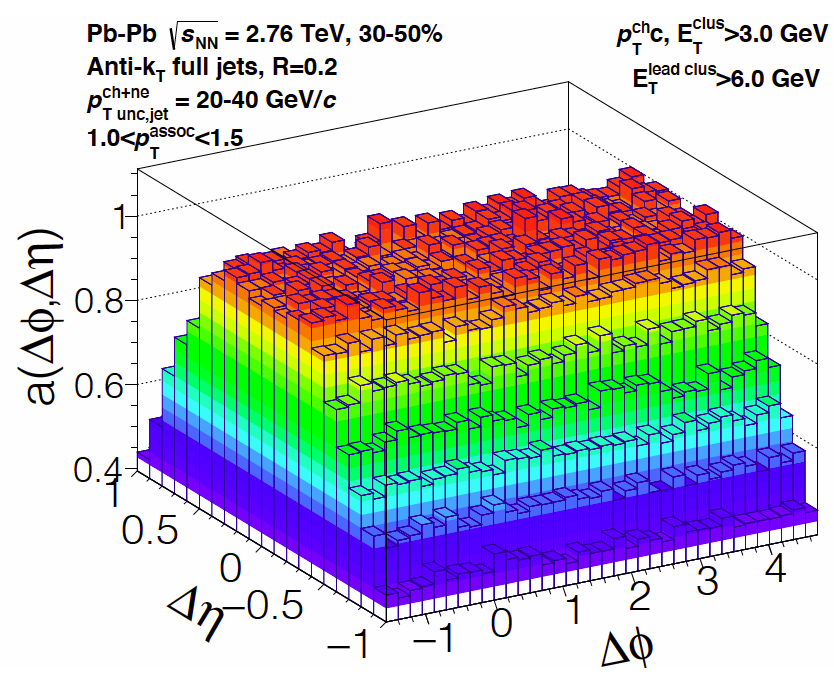
\includegraphics[width=0.7\textwidth]{figure/samplefig1.png}
	\caption{A sample figure to show}
\end{figure}

공개하지 아니한 회의내용의 공표에 관하여는 법률이 정하는 바에 의한다. 지방자치단체는 주민의 복리에 관한 사무를 처리하고 재산을 관리하며, 법령의 범위안에서 자치에 관한 규정을 제정할 수 있다. 대법원은 법률에 저촉되지 아니하는 범위안에서 소송에 관한 절차, 법원의 내부규율과 사무처리에 관한 규칙을 제정할 수 있다. 대통령은 조약을 체결·비준하고, 외교사절을 신임·접수 또는 파견하며, 선전포고와 강화를 한다. 예비비는 총액으로 국회의 의결을 얻어야 한다. 예비비의 지출은 차기국회의 승인을 얻어야 한다. 형사피고인은 유죄의 판결이 확정될 때까지는 무죄로 추정된다. 대한민국의 주권은 국민에게 있고, 모든 권력은 국민으로부터 나온다.

\subsubsection{헌법재판소의 위헌판결과 국민투표}

명령·규칙 또는 처분이 헌법이나 법률에 위반되는 여부가 재판의 전제가 된 경우에는 대법원은 이를 최종적으로 심사할 권한을 가진다. 계엄을 선포한 때에는 대통령은 지체없이 국회에 통고하여야 한다. 대통령은 필요하다고 인정할 때에는 외교·국방·통일 기타 국가안위에 관한 중요정책을 국민투표에 붙일 수 있다. 국방상 또는 국민경제상 긴절한 필요로 인하여 법률이 정하는 경우를 제외하고는, 사영기업을 국유 또는 공유로 이전하거나 그 경영을 통제 또는 관리할 수 없다. 대통령은 제1항과 제2항의 처분 또는 명령을 한 때에는 지체없이 국회에 보고하여 그 승인을 얻어야 한다. 군사법원의 조직·권한 및 재판관의 자격은 법률로 정한다.

\subsubsection{대법원장 임명과 임기}

대법원장의 임기는 6년으로 하며, 중임할 수 없다. 새로운 회계연도가 개시될 때까지 예산안이 의결되지 못한 때에는 정부는 국회에서 예산안이 의결될 때까지 다음의 목적을 위한 경비는 전년도 예산에 준하여 집행할 수 있다. 국회는 의장 1인과 부의장 2인을 선출한다. 모든 국민의 재산권은 보장된다. 그 내용과 한계는 법률로 정한다. 국민경제의 발전을 위한 중요정책의 수립에 관하여 대통령의 자문에 응하기 위하여 국민경제자문회의를 둘 수 있다. 근로조건의 기준은 인간의 존엄성을 보장하도록 법률로 정한다. 위원은 정당에 가입하거나 정치에 관여할 수 없다. 헌법재판소는 법률에 저촉되지 아니하는 범위안에서 심판에 관한 절차, 내부규율과 사무처리에 관한 규칙을 제정할 수 있다.

\subsection{국무총리와 국무위원의 해임}

국회는 국무총리 또는 국무위원의 해임을 대통령에게 건의할 수 있다. 대법원장은 국회의 동의를 얻어 대통령이 임명한다. 국가는 여자의 복지와 권익의 향상을 위하여 노력하여야 한다. 나는 헌법을 준수하고 국가를 보위하며 조국의 평화적 통일과 국민의 자유와 복리의 증진 및 민족문화의 창달에 노력하여 대통령으로서의 직책을 성실히 수행할 것을 국민 앞에 엄숙히 선서합니다. 국가는 건전한 소비행위를 계도하고 생산품의 품질향상을 촉구하기 위한 소비자보호운동을 법률이 정하는 바에 의하여 보장한다. 모든 국민은 법률이 정하는 바에 의하여 납세의 의무를 진다. 대법관의 임기는 6년으로 하며, 법률이 정하는 바에 의하여 연임할 수 있다.

\chapter{사면과 복권}

사면·감형 및 복권에 관한 사항은 법률로 정한다. 선거에 있어서 최고득표자가 2인 이상인 때에는 국회의 재적의원 과반수가 출석한 공개회의에서 다수표를 얻은 자를 당선자로 한다. 정부는 회계연도마다 예산안을 편성하여 회계연도 개시 90일전까지 국회에 제출하고, 국회는 회계연도 개시 30일전까지 이를 의결하여야 한다. 국회는 국가의 예산안을 심의·확정한다. 국회의원은 법률이 정하는 직을 겸할 수 없다. 국가안전보장회의는 대통령이 주재한다. 교육의 자주성·전문성·정치적 중립성 및 대학의 자율성은 법률이 정하는 바에 의하여 보장된다. 대통령은 국가의 독립·영토의 보전·국가의 계속성과 헌법을 수호할 책무를 진다.

국가원로자문회의의 의장은 직전대통령이 된다. 다만, 직전대통령이 없을 때에는 대통령이 지명한다. 선거에 관한 경비는 법률이 정하는 경우를 제외하고는 정당 또는 후보자에게 부담시킬 수 없다. 국회는 의원의 자격을 심사하며, 의원을 징계할 수 있다. 국가안전보장에 관련되는 대외정책·군사정책과 국내정책의 수립에 관하여 국무회의의 심의에 앞서 대통령의 자문에 응하기 위하여 국가안전보장회의를 둔다. 국가는 법률이 정하는 바에 의하여 재외국민을 보호할 의무를 진다. 비상계엄이 선포된 때에는 법률이 정하는 바에 의하여 영장제도, 언론·출판·집회·결사의 자유, 정부나 법원의 권한에 관하여 특별한 조치를 할 수 있다.

\begin{figure}[!h]
	\centering
	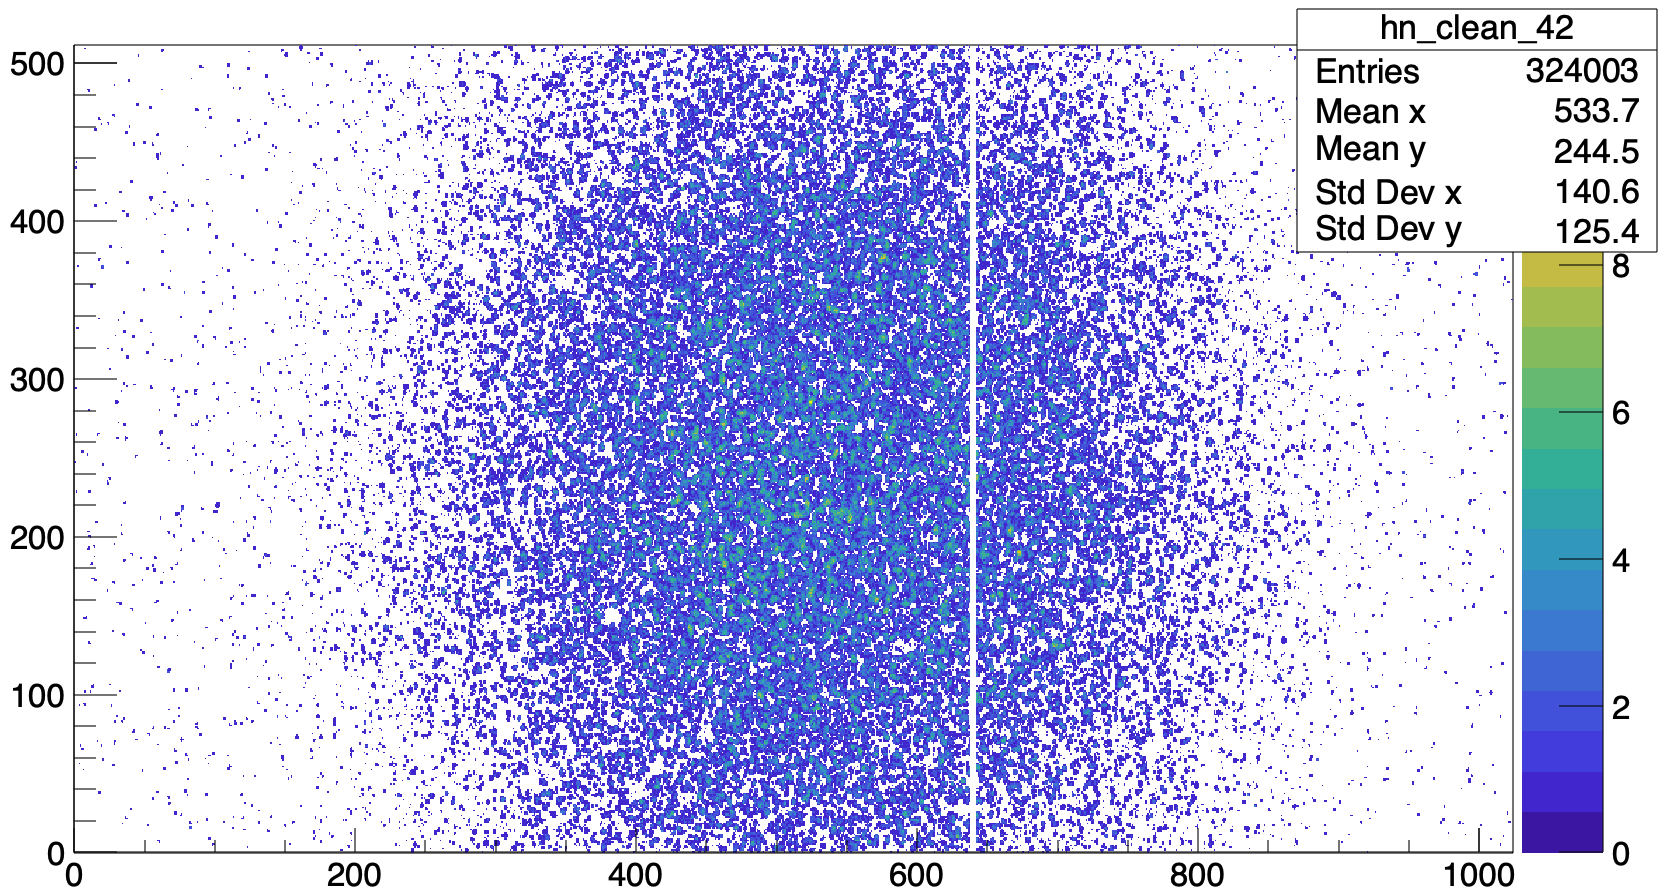
\includegraphics[width=0.7\textwidth]{figure/samplefig2.png}
	\caption{A 2nd figure to show}
\end{figure}

%
% 참고문헌
%

\begin{thebibliography}{00}
	\bibitem{item1} Reference 1
	\bibitem{item2} Reference 2
	\bibitem{item3} Reference 3
\end{thebibliography}

\appendix
\chapter{대통령의 겸직금지}

대통령은 국무총리·국무위원·행정각부의 장 기타 법률이 정하는 공사의 직을 겸할 수 없다. 정당의 설립은 자유이며, 복수정당제는 보장된다. 군인 또는 군무원이 아닌 국민은 대한민국의 영역안에서는 중대한 군사상 기밀·초병·초소·유독음식물공급·포로·군용물에 관한 죄중 법률이 정한 경우와 비상계엄이 선포된 경우를 제외하고는 군사법원의 재판을 받지 아니한다. 모든 국민은 행위시의 법률에 의하여 범죄를 구성하지 아니하는 행위로 소추되지 아니하며, 동일한 범죄에 대하여 거듭 처벌받지 아니한다. 국회의원은 현행범인인 경우를 제외하고는 회기중 국회의 동의없이 체포 또는 구금되지 아니한다.

국회는 헌법개정안이 공고된 날로부터 60일 이내에 의결하여야 하며, 국회의 의결은 재적의원 3분의 2 이상의 찬성을 얻어야 한다. 정부는 예산에 변경을 가할 필요가 있을 때에는 추가경정예산안을 편성하여 국회에 제출할 수 있다. 대한민국은 민주공화국이다. 사회적 특수계급의 제도는 인정되지 아니하며, 어떠한 형태로도 이를 창설할 수 없다. 국회는 상호원조 또는 안전보장에 관한 조약, 중요한 국제조직에 관한 조약, 우호통상항해조약, 주권의 제약에 관한 조약, 강화조약, 국가나 국민에게 중대한 재정적 부담을 지우는 조약 또는 입법사항에 관한 조약의 체결·비준에 대한 동의권을 가진다. 국가는 농업 및 어업을 보호·육성하기 위하여 농·어촌종합개발과 그 지원등 필요한 계획을 수립·시행하여야 한다.

\pagebreak
\acknowledgement %감사의 글을 작성하지 않을경우 삭제가능

국회는 헌법개정안이 공고된 날로부터 60일 이내에 의결하여야 하며, 국회의 의결은 재적의원 3분의 2 이상의 찬성을 얻어야 한다. 정부는 예산에 변경을 가할 필요가 있을 때에는 추가경정예산안을 편성하여 국회에 제출할 수 있다. 대한민국은 민주공화국이다. 사회적 특수계급의 제도는 인정되지 아니하며, 어떠한 형태로도 이를 창설할 수 없다. 국회는 상호원조 또는 안전보장에 관한 조약, 중요한 국제조직에 관한 조약, 우호통상항해조약, 주권의 제약에 관한 조약, 강화조약, 국가나 국민에게 중대한 재정적 부담을 지우는 조약 또는 입법사항에 관한 조약의 체결·비준에 대한 동의권을 가진다. 국가는 농업 및 어업을 보호·육성하기 위하여 농·어촌종합개발과 그 지원등 필요한 계획을 수립·시행하여야 한다.

대법원에 대법관을 둔다. 다만, 법률이 정하는 바에 의하여 대법관이 아닌 법관을 둘 수 있다. 법률이 헌법에 위반되는 여부가 재판의 전제가 된 경우에는 법원은 헌법재판소에 제청하여 그 심판에 의하여 재판한다. 모든 국민은 근로의 권리를 가진다. 국가는 사회적·경제적 방법으로 근로자의 고용의 증진과 적정임금의 보장에 노력하여야 하며, 법률이 정하는 바에 의하여 최저임금제를 시행하여야 한다. 대통령은 내란 또는 외환의 죄를 범한 경우를 제외하고는 재직중 형사상의 소추를 받지 아니한다. 국가는 평생교육을 진흥하여야 한다. 국가는 과학기술의 혁신과 정보 및 인력의 개발을 통하여 국민경제의 발전에 노력하여야 한다.

헌법재판소의 조직과 운영 기타 필요한 사항은 법률로 정한다. 국무위원은 국정에 관하여 대통령을 보좌하며, 국무회의의 구성원으로서 국정을 심의한다. 국채를 모집하거나 예산외에 국가의 부담이 될 계약을 체결하려 할 때에는 정부는 미리 국회의 의결을 얻어야 한다. 피고인의 자백이 고문·폭행·협박·구속의 부당한 장기화 또는 기망 기타의 방법에 의하여 자의로 진술된 것이 아니라고 인정될 때 또는 정식재판에 있어서 피고인의 자백이 그에게 불리한 유일한 증거일 때에는 이를 유죄의 증거로 삼거나 이를 이유로 처벌할 수 없다. 대통령은 전시·사변 또는 이에 준하는 국가비상사태에 있어서 병력으로써 군사상의 필요에 응하거나 공공의 안녕질서를 유지할 필요가 있을 때에는 법률이 정하는 바에 의하여 계엄을 선포할 수 있다.

이 헌법은 1988년 2월 25일부터 시행한다. 다만, 이 헌법을 시행하기 위하여 필요한 법률의 제정·개정과 이 헌법에 의한 대통령 및 국회의원의 선거 기타 이 헌법시행에 관한 준비는 이 헌법시행 전에 할 수 있다. 공무원인 근로자는 법률이 정하는 자에 한하여 단결권·단체교섭권 및 단체행동권을 가진다. 사법권은 법관으로 구성된 법원에 속한다. 국토와 자원은 국가의 보호를 받으며, 국가는 그 균형있는 개발과 이용을 위하여 필요한 계획을 수립한다. 공무원의 직무상 불법행위로 손해를 받은 국민은 법률이 정하는 바에 의하여 국가 또는 공공단체에 정당한 배상을 청구할 수 있다. 이 경우 공무원 자신의 책임은 면제되지 아니한다.

대통령은 헌법과 법률이 정하는 바에 의하여 공무원을 임면한다. 모든 국민은 신속한 재판을 받을 권리를 가진다. 형사피고인은 상당한 이유가 없는 한 지체없이 공개재판을 받을 권리를 가진다. 헌법재판소 재판관은 정당에 가입하거나 정치에 관여할 수 없다. 공무원의 신분과 정치적 중립성은 법률이 정하는 바에 의하여 보장된다. 국가의 세입·세출의 결산, 국가 및 법률이 정한 단체의 회계검사와 행정기관 및 공무원의 직무에 관한 감찰을 하기 위하여 대통령 소속하에 감사원을 둔다. 국가는 청원에 대하여 심사할 의무를 진다. 모든 국민은 그 보호하는 자녀에게 적어도 초등교육과 법률이 정하는 교육을 받게 할 의무를 진다.

국무위원은 국무총리의 제청으로 대통령이 임명한다. 이 헌법공포 당시의 국회의원의 임기는 제1항에 의한 국회의 최초의 집회일 전일까지로 한다. 국가안전보장회의의 조직·직무범위 기타 필요한 사항은 법률로 정한다. 모든 국민은 법률이 정하는 바에 의하여 국방의 의무를 진다. 대통령의 임기가 만료되는 때에는 임기만료 70일 내지 40일전에 후임자를 선거한다. 대통령이 제1항의 기간내에 공포나 재의의 요구를 하지 아니한 때에도 그 법률안은 법률로서 확정된다. 국회의원의 수는 법률로 정하되, 200인 이상으로 한다. 체포·구속·압수 또는 수색을 할 때에는 적법한 절차에 따라 검사의 신청에 의하여 법관이 발부한 영장을 제시하여야 한다. 다만, 현행범인인 경우와 장기 3년 이상의 형에 해당하는 죄를 범하고 도피 또는 증거인멸의 염려가 있을 때에는 사후에 영장을 청구할 수 있다.

행정권은 대통령을 수반으로 하는 정부에 속한다. 국회의원이 회기전에 체포 또는 구금된 때에는 현행범인이 아닌 한 국회의 요구가 있으면 회기중 석방된다. 제3항의 승인을 얻지 못한 때에는 그 처분 또는 명령은 그때부터 효력을 상실한다. 이 경우 그 명령에 의하여 개정 또는 폐지되었던 법률은 그 명령이 승인을 얻지 못한 때부터 당연히 효력을 회복한다. 모든 국민은 헌법과 법률이 정한 법관에 의하여 법률에 의한 재판을 받을 권리를 가진다. 법관은 헌법과 법률에 의하여 그 양심에 따라 독립하여 심판한다. 외국인은 국제법과 조약이 정하는 바에 의하여 그 지위가 보장된다. 정기회의 회기는 100일을, 임시회의 회기는 30일을 초과할 수 없다.

대통령은 국회에 출석하여 발언하거나 서한으로 의견을 표시할 수 있다. 훈장등의 영전은 이를 받은 자에게만 효력이 있고, 어떠한 특권도 이에 따르지 아니한다. 대통령은 제3항과 제4항의 사유를 지체없이 공포하여야 한다. 대한민국은 통일을 지향하며, 자유민주적 기본질서에 입각한 평화적 통일 정책을 수립하고 이를 추진한다. 국군은 국가의 안전보장과 국토방위의 신성한 의무를 수행함을 사명으로 하며, 그 정치적 중립성은 준수된다. 제2항과 제3항의 처분에 대하여는 법원에 제소할 수 없다. 국회는 선전포고, 국군의 외국에의 파견 또는 외국군대의 대한민국 영역안에서의 주류에 대한 동의권을 가진다.

\end{document}